%% LyX 2.1.4 created this file.  For more info, see http://www.lyx.org/.
%% Do not edit unless you really know what you are doing.
\documentclass[11pt,czech,american]{book}
\usepackage[T1]{fontenc}
\usepackage[utf8]{inputenc}
\usepackage[a4paper]{geometry}
\geometry{verbose,tmargin=4cm,bmargin=3cm,lmargin=3cm,rmargin=2cm,headheight=0.8cm,headsep=1cm,footskip=0.5cm}
\pagestyle{headings}
\setcounter{secnumdepth}{3}
\usepackage{url}
\usepackage{amsmath}
\usepackage{amsthm}
\usepackage{amssymb}
\usepackage{graphicx}
\usepackage{setspace}
\usepackage[final]{pdfpages}
\usepackage{natbib}
\usepackage{mathrsfs}
\usepackage{algorithm}
\usepackage{algorithmicx}
\usepackage[noend]{algpseudocode}
\usepackage{caption}


\usepackage{array}
\usepackage{ragged2e}

\usepackage{lipsum}
\usepackage{psvectorian}

\DeclareMathOperator*{\argmax}{arg\,max}

\makeatletter
%%%%%%%%%%%%%%%%%%%%%%%%%%%%%% Textclass specific LaTeX commands.
\newenvironment{lyxlist}[1]
{\begin{list}{}
{\settowidth{\labelwidth}{#1}
 \setlength{\leftmargin}{\labelwidth}
 \addtolength{\leftmargin}{\labelsep}
 \renewcommand{\makelabel}[1]{##1\hfil}}}
{\end{list}}

%%%%%%%%%%%%%%%%%%%%%%%%%%%%%% User specified LaTeX commands.
%% Font setup: please leave the LyX font settings all set to 'default'
%% if you want to use any of these packages:

%% Use Times New Roman font for text and Belleek font for math
%% Please make sure that the 'esint' package is turned off in the
%% 'Math options' page.
\usepackage[varg]{txfonts}

%% Use Utopia text with Fourier-GUTenberg math
%\usepackage{fourier}

%% Bitstream Charter text with Math Design math
%\usepackage[charter]{mathdesign}

%%---------------------------------------------------------------------

%% Make the multiline figure/table captions indent so that the second
%% line "hangs" right below the first one.
%\usepackage[format=hang]{caption}

%% Indent even the first paragraph in each section
\usepackage{indentfirst}

%%---------------------------------------------------------------------

%% Disable page numbers in the TOC. LOF, LOT (TOC automatically
%% adds \thispagestyle{chapter} if not overriden
%\addtocontents{toc}{\protect\thispagestyle{empty}}
%\addtocontents{lof}{\protect\thispagestyle{empty}}
%\addtocontents{lot}{\protect\thispagestyle{empty}}

%% Shifts the top line of the TOC (not the title) 1cm upwards 
%% so that the whole TOC fits on 1 page. Additional page size
%% adjustment is performed at the point where the TOC
%% is inserted.
%\addtocontents{toc}{\protect\vspace{-1cm}}

%%---------------------------------------------------------------------

% completely avoid orphans (first lines of a new paragraph on the bottom of a page)
\clubpenalty=9500

% completely avoid widows (last lines of paragraph on a new page)
\widowpenalty=9500

% disable hyphenation of acronyms
\hyphenation{CDFA HARDI HiPPIES IKEM InterTrack MEGIDDO MIMD MPFA DICOM ASCLEPIOS MedInria}

%%---------------------------------------------------------------------

%% Print out all vectors in bold type instead of printing an arrow above them
\renewcommand{\vec}[1]{\boldsymbol{#1}}

% Replace standard \cite by the parenthetical variant \citep
%\renewcommand{\cite}{\citep}

\makeatother

\usepackage{babel}

\newcommand{\ornamentleft}{%
	\psvectorian[width=2em]{2}%
}
\newcommand{\ornamentright}{%
	\psvectorian[width=2em,mirror]{2}%
}

\newcommand{\ornamentheader}[1]{%
	\begin{center}
		\ornamentleft
		\quad{\large\emph{#1}}\quad % style as desired
		\ornamentright
	\end{center}%
}

\newlength{\rlength}\setlength{\rlength}{16cm}
\newcommand{\ruletext}[2][\rlength]{%
	\noindent%
	\parbox{#1}{%
		\noindent\dotfill\raisebox{-.3\ht\strutbox}{#2}\dotfill\par}%
}





\begin{document}
\def\documentdate{July 7, 2017}

\newtheorem{definition}{Definition}[chapter]
\newtheorem{note}{Note}[chapter]
\newtheorem{example}{Example} 
\newtheorem{assumption}{Assumption} 

\newtheorem{theorem}{Theorem}
\newtheorem*{remark}{Remark}

\captionsetup[figure]{labelfont={bf},labelformat={default},labelsep=period,name={Fig.}}


\def\documentdate{\today}

\pagestyle{empty}
{\centering

\noindent %
\begin{minipage}[c]{3cm}%
\noindent \begin{center}

\includegraphics[width=3cm,height=3cm,keepaspectratio]{Images/TITLE/cvut}
\par\end{center}%
\end{minipage}%
\begin{minipage}[c]{0.6\linewidth}%
\begin{center}
\textsc{\large{}Czech Technical University in Prague}{\large{}}\\
{\large{}Faculty of Nuclear Sciences and Physical Engineering}
\par\end{center}%
\end{minipage}%
\begin{minipage}[c]{3cm}%
\noindent \begin{center}

\includegraphics[width=3cm,height=3cm,keepaspectratio]{Images/TITLE/fjfi}
\par\end{center}%
\end{minipage}

\vspace{3cm}


\textbf{\huge{}Real Options Valuation: A Dynamic Programming Approach}{\huge \par}

\vspace{1cm}


\selectlanguage{czech}%
\textbf{\huge{}Oceňování projektů metodou reálných opcí z pohledu dynamického progamování}{\huge \par}

\selectlanguage{american}%
\vspace{2cm}


{\large{}Master's Thesis}{\large \par}

}

\vfill{}

\begin{lyxlist}{MMMMMMMMM}
\begin{singlespace}
\item [{Author:}] \textbf{Filip Rolenec}
\item [{Supervisor:}] \textbf{Ing. Rudolf Kulhavý, DrSc.}
\end{singlespace}

\item [{Language~advisor:}] \textbf{Ing. Rudolf Kulhavý, DrSc.} 
\begin{singlespace}
\item [{Academic~year:}] 2020/2021\end{singlespace}

\end{lyxlist}
\newpage{}

~\newpage{}

~

\vfill{}


\begin{center}
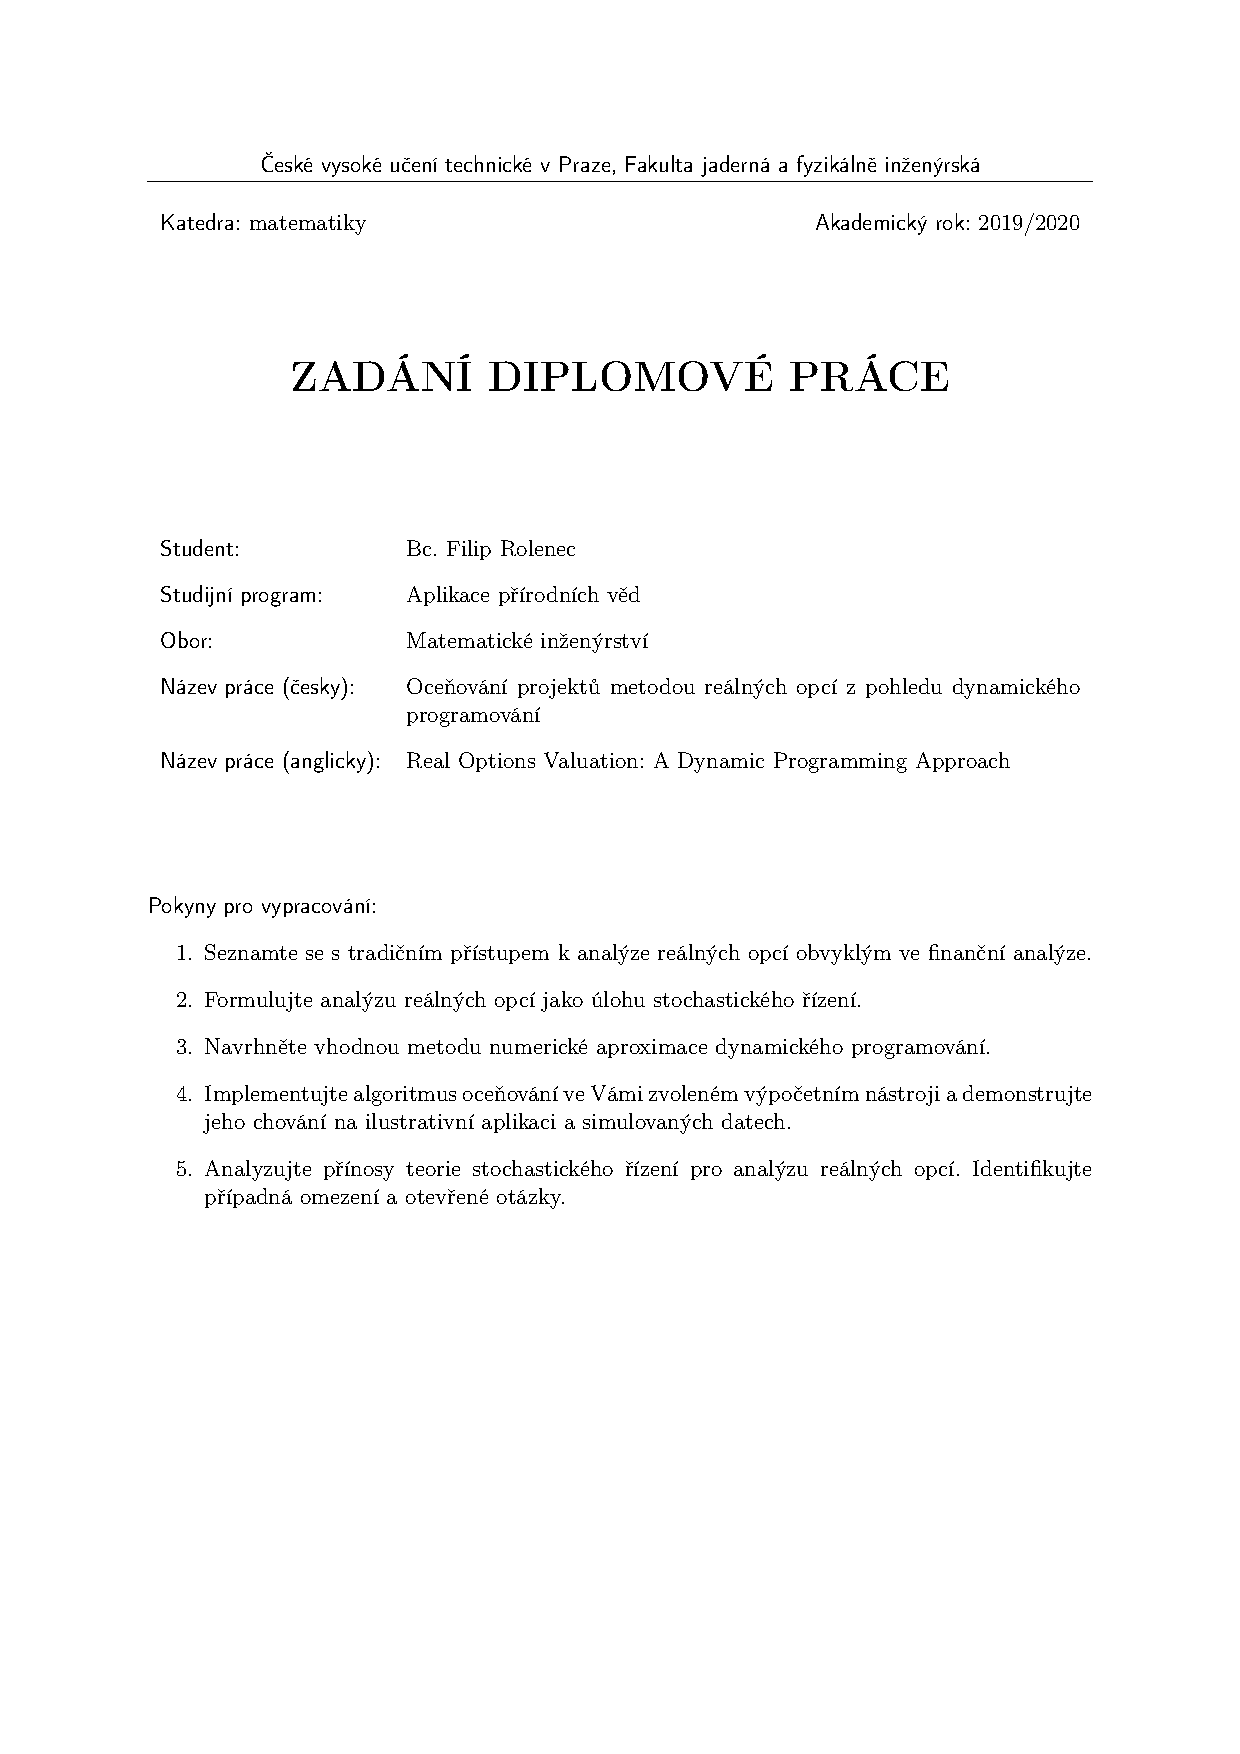
\includepdf[pages={1}]{Images/zadaniMT.pdf}


\par\end{center}

\vfill{}


~\newpage{}

~

\vfill{}


\begin{center}
\includepdf[pages={2}]{Images/zadaniMT.pdf}
\par\end{center}

\vfill{}


~\newpage{}

\noindent \emph{\Large{}Acknowledgment:}{\Large \par}

\noindent I would like to thank my supervisor Ing. Rudolf Kulhavý, DrSc. for his professional guidance and all the advice given while creating this thesis. 

\vfill

\noindent \emph{\Large{}Author's declaration:}{\Large \par}

\noindent I declare that this Master's thesis is entirely
my own work and I have listed all the used sources in the bibliography.

\bigskip{}


\noindent Prague, \documentdate\hfill{}Filip Rolenec

\vspace{2cm}


\newpage{}

~\newpage{}

\selectlanguage{czech}%
\begin{onehalfspace}
\noindent \emph{Název práce:}

\noindent \textbf{Oceňování projektů metodou reálných opcí z pohledu dynamického progamování}
\end{onehalfspace}

\bigskip{}


\noindent \emph{Autor:} Filip Rolenec

\bigskip{}


\noindent \emph{Obor:} Matematické inženýrství 


\bigskip{}


\noindent \emph{Druh práce:} Diplomová práce

\bigskip{}


\noindent \emph{Vedoucí práce:} Ing. Rudolf Kulhavý, DrSc.


\bigskip{}


\noindent \emph{Abstrakt:} Investiční příležitosti jsou v současné době oceňovány pomocí řady algoritmů a metrik vzešlých z ekonomické teorie. Nejčastěji používaná metoda \textit{diskontovaných peněžních toků} (DCF) zohledňuje časovou hodnotu peněz a pro jednoduché projekty dává investorům velmi dobré odhady s minimálními požadavky na matematické znalosti. Složitější projekty, které v této práci chápeme jako projekty s vysokou mírou neurčitosti a existencí následných manažerských rozhodnutí, je možné oceňovat pomocí teorie \textit{reálných opcí} (ROA). Metoda ROA vychází z nedokonalé analogie oceňování finančních opcí a přiznává hodnotu možnostem změny projektového plánu. 

Tato práce má za cíl představit nový rámec pro oceňování investičních příležitostí, jejichž řízení je chápáno  jako stochastický rozhodovací problém. Tento rámec, umožňující využití desítek let výzkumu v oblasti stochastické rozhodovací teorie, pokrývá metody DCF a ROA, přičemž zjemňuje jejich předpoklady. Hlavní přínosy nového oceňovacího rámce jsou: možnost zodhlednění více zdrojů neurčitosti, modelování neurčitosti libovolnou distribucí, přímočaré začlenění bayesovského učení, modelování přístupu k riziku rozhodovacího subjektu a libovolný počet i druh povolených manažerských akcí. 

Nový rámec znatelně rozšiřuje třídu projektů ocenitelných s velkou přesností a lze ho chápat jako sjednocující zobecnění technik oceňování v podnikovém řízení. 


\bigskip{}


\noindent \emph{Klíčová slova:}   Analýza reálných opcí, Black-Scholes model, Diskontované peněžní toky, Dynamické programování, Energetika, Oceňování projektů, Stochastické řízení



\selectlanguage{american}%
\vfill{}
~

\begin{onehalfspace}
\noindent \emph{Title:}

\noindent \textbf{Real Options Valuation: A Dynamic Programming Approach}
\end{onehalfspace}

\bigskip{}


\noindent \emph{Author:} Filip Rolenec

\bigskip{}


\noindent \emph{Abstract:} The valuation of investment opportunities is currently done via metrics and algorithms formed by the economical theory. The majority of investors and companies still values projects with a method of \textit{discounted cash flows} (DCF), which takes into account the time value of money and gives solid results for simple projects with minimal requirement on mathematical skills. More complicated projects, which are in this thesis thought of as projects with a substantial degree of inner uncertainty and with an existence of further managerial decisions, can be valued by the \textit{real options analysis} (ROA). This method comes from an imperfect analogy to financial option valuation and it recognizes the value of the ability to change the course of a given project.  

This thesis presents a new valuation framework for projects, which are understood as problems of optimal stochastic decision control. This framework incorporates the DCF and ROA methods, simplifies the requested assumptions and allows for decades of research in the field of \textit{stochastic decision theory} (SDT) to be used. The main contributions of the new framework are: ability to incorporate multiple sources of uncertainty, usage of any distribution for modeling the uncertainty, ability to conveniently incorporate Bayesian learning, ability to model user's approach to risk and ability to model any type and scale of managerial actions.

The new framework significantly expands the class of projects that can be reasonably valued and it can be understood as a unification of project valuation in business management.


\bigskip{}


\noindent \emph{Keywords:} Black-Scholes model, Discounted cash flow, Dynamic programming, Power industry, Project valuation,  Real option analysis, Stochastic decision control

\newpage{}

~\newpage{}

\pagestyle{plain}

\tableofcontents{}

\newpage{}


\chapter{Introduction}
The ability to systematically and reliably value projects is the core of investment decision making. According to the economical theory presented by \cite{} \footnote{That guy from Duke university} profits of an investment reflect the value added to the participants of the market, expressed by actual spending of their money. The profits of a venture are understood as the ultimate measure of additional value that has been created. 

A good valuation technique enables companies to increase their profits and as \cite{BerDeM:09} (?)  says: the main and actually only goal of a manager is to increase the wealth of stakeholders. It is thus rather fortunate that, by the logic of \cite{} \footnote{Guy from duke}, in free market, increasing this value coincides with the adding value to all interested participants on the market. One could thus extrapolate and say, that in free market, the goal of a manager is to improve lives of market participants. 

The current state of capital investment valuation techniques is very diverse. Majority of investors rely predominantly on the standard Net Present Value (NPV) technique, its generalization in a form of NPV with scenarios (sometimes called Decision Tree Analysis(DTA)) or NPV-derived metrics with some mostly artificial parameters, such as NPV with Risk Adjusted Discount Rate (RADR) or Internal Rate of Return (IRR). \footnote{Create citations to these statements}

These valuation techniques are usually simple, resulting in a very limited scope of their application. Two main problems are that they do not address the problem of uncertainty or further management ability, in much detail, or in the case of uncertainty the argumentation is misleading \footnote{Risky FCFs should be discounted more...}.

In many articles and economical books one superior valuation technique, that recognizes the value of further managerial actions and also copes with the uncertainty in more complex way is cal Real Options Analysis (ROA). Project valuation by ROA is in literature used in three forms, differing in the level of its analogy to valuation of financial options, which is elegantly handled by the Black-Sholes-Merton Nobel prize winning valuation technique \cite{}. 

The value added by recognizing the importance of further management in projects with high degree of uncertainty is significant. Articles \cite{} and \cite{} show, how standard valuation techniques tend to undervalue these projects, leading to potentially significant unrealized profits. 

The core of BSM model, and thus its analogy in the form of ROA, is only an argument about the expected value of a price, which is understood as following log-normally distributed random process. This argument is used in creation of so called risk-neutral probabilities of price movements of the underlying variable. 

By reading the publications about ROA one starts to be accustomed to the structure of projects as a collection of managerial decisions. This narrative rings a strong bell to a scholar that has encountered stochastic decision theory (SDT). 

Stochastic decision theory, with its decades of research, offers a brilliant framework for any decision making problem, which projects effectively are. The analogy for project value has also a potential to be found in the value functions which represent the expected cumulative rewards from undertaking the optimal strategy. 

The goal of this thesis is to incorporate some key features of economical thinking about value of a project in the framework of SDT. The main focus in put on the approach to risk, time value of money and enabling for multiple sources of risk in the models. 

The first dimension of risk - uncertainty about the monetary outcome - in the economical theory is being in SDT addressed by the utility theory. The second dimension - assessing different values to assets based on their correlation to the overall market - has no clear analogy with the SDT theory, which is solved by making the utility function two-dimensional, or in a case of small number of different correlations, multiple utility functions with subscripts are defined. 

The time value of money exists in SDT in a simple form of discounting, which is very similar to discounting with either risk-free discount rate, or risk-adjusted discount rate in economics. In this thesis the idea of people being logically indifferent to some sums of money now and in the future based on their current assets and ability to borrow and invest with no risk is presented. 

In addition to being able to interpret the classical valuation techniques in the form of SDT, this new approach allows us to present theoretically any number of different uncertainties modeled by any random process (the economical theory exclusively uses normal and log-normal processes). 

Because the project is modeled by the SDT framework, its value is assessed through the process of dynamic programming - in a case of simple models - or by the advanced theory of approximate dynamic programming (ADP) - in case of more complicated models. 

The advantages of understanding a project's valuation problem as a dynamic decision problems are then demonstrated on two examples of business areas with multiple sources of production. Examples of such business are producers of electric power, water, raw materials that can be extracted by multiple viable methods, public transportation companies and others. 

This class of business was chosen due to the variability in available production units of a given material/service and partially due to the some level of author's expertise in the field of power generation. 

First, it is shown that the formulation of ROA from authors like Guthrie \cite{Gut:09}, Vollert \cite{Vol:03} and others \cite{} can be interpreted by SDT rather easily, smoothly allowing for multiple sources and models of uncertainty, possibility of Bayesian learning and the ability to cope with high dimensional problems. 

Second a possible generalization of the example is shown, presenting the full power of the new approach. It is expected that by lowering the assumptions of ROA and similar techniques, considering various aspects of project's features with less approximation, a more precise valuation can be achieved. 

The advantage of SDT formulation in comparison to ROA and other models is not as clear-cut as the ROA vs NPV for example, where NPV serves only a lower bound to ROA valuation. The SDT approach tries to incorporate as much information as possible to get the most precise current value of a project, which does not have to be same or higher as ROA. 

The new SDT approach has a goal to incorporate all the standard economical theory, approach to risk, time value of money, different valuation of returns on market-correlated assets, while enabling more complex modeling of uncertainty, Bayesian learning and a way to address projects, that translate to a high-dimensional decision problems. 

\textbf{Suggestions: ROA history, more citations, talking about replicating portfolios}



%\addcontentsline{toc}{chapter}{Introduction}

%\addcontentsline{toc}{chapter}{Preliminaries}

\pagestyle{headings}




\chapter{Preliminaries}
\ruletext{Introduction to preliminaries}

To properly understand a mathematical text it is important to first define the used notions and symbolism. Since this thesis is based on many different authors, from both financial and mathematical world, a short unifying overview of the used theory is important. 

The notation used in this thesis comes predominantly from the most influential authors in the respective fields of study: 
\begin{itemize}
	\item general economy \cite{BerDeM:09};
	\item real options \cite{Gut:09};
	\item stochastic decision theory \cite{BacChi:19}.
\end{itemize}

 The pure mathematical symbolism comes from the author's studying experience at FNSPE CTU and its applicability is proven in his previous works \cite{Rol:18} and \cite{Rol:19}. 
\footnote{Filip == Author or Filip == I/Me} 

\ruletext{}
\section{Used mathematical symbolism}
\ruletext{Sets, random variables, what do I mean by 'probability'}

In the whole thesis, bold capital letters, such as $\mathbf{X}$, represent a set of all elements $x \in \mathbf{X}$ as in \cite{Rol:18}. The cardinality of a set $\mathbf{X}$ is denoted with two vertical lines as $|\mathbf{X}|$. Random variables, understood in a sense of the standard Kolmogorov's probability theory \cite{Kol:60}\footnote{Does this citation make sense? }, are represented with a tilde above the variable, i.e. $\tilde{x}$. Realizations of random variables are denoted by the same letters as the random variable without the tilde, i.e. $x$. 

\begin{definition}(Probability)
	Let $\tilde{x}$ be a random discrete variable. Then $P(x)$ denotes a probability that the realization of $\tilde{x}=x$. Similarly if $\tilde{x}$ is a continuous random variable, then $p(x)$ denotes a probability density of the realization $\tilde{x}=x$. 
\end{definition}
\begin{remark}
	To rigorously unify the notation and simplify the formulas a Radon-Nikodým (RN) density \cite{Rao:87a} is introduced  with the notation $p(x)$ and the name ``probability density``. The dominating measure of this RN density is either the counting measure (in discrete case) or a the Lebesgue measure (in continuous case). The notation $P(X)$ is reserved only for the cases when the discreteness of the argument needs to be emphasized. 
\end{remark}

The last general definition is the definition of well known concept of conditional probability \cite{Jay:03}. 
\begin{definition}(Conditional probability)
	Let, depending on the context, symbol $p(x|y)$ represents either the conditional probability on discrete variables or the conditional probability density on continuous variables. Then the $p(x|y)$ is defined as:
	\begin{equation}\label{eq:condP}
	p(x|y)=\frac{p(x,y)}{p(y)},
	\end{equation} where $p(x,y)$ is a joint probability density of $x$ and $y$. 
\end{definition}

\begin{remark}
	The definition of conditional probability expressed by the equation (\ref{eq:condP}) corresponds with the classic definitions of the conditional probability and conditional probability density in both the discrete and continuous case. 
\end{remark}

<Probably some other definitions that will be needed in the following chapters> 

\ruletext{}

\section{General economics}
\ruletext{Introduction and basic financial concepts. }

This thesis is built on two main theoretical pillars, the theory of corporate finance \cite{BerDeM:09} and stochastic decision theory (SDT) \cite{BacChi:19}. A basic review of corporate finance terminology and procedures is presented in this section with a focus on project valuation techniques. 


\begin{definition}[Project]
	A project is defined as a piece of planned work or an activity that is finished over a period of time and intended to achieve a particular purpose, mainly a wealth increase of a company or an individual. \footnote{First part comes from Cambridge dictionary. Is that ok just to cite it? }
\end{definition}

\begin{definition}[Value]
	The amount of money that can be received for something. \footnote{Again cambridge dictionary...} \footnote{This definition is added to say that by value in economics we mean money that we can obtain from the asset.}
\end{definition}

A value of a project is naturally a function of realized elementary monetary transactions within the project and the potential selling price of remaining assets. To track and model each transaction of a project in detail is in principle possible, but such approach would be way too complex for practical usage. Furthermore, its benefits would most likely not be significant enough to defend the extra effort of decision makers. 


For purposes of project valuation an aggregation of elementary monetary transactions - a concept of cash flow (CF) and free cash flow (FCF) are used in the world of corporate finance. 

\begin{definition}(Cash flow)
	Cash flow is the net amount of cash and cash-equivalents being transferred into and out of a business (project).  \footnote{Investopedia, economical books do not define it. }
	
\end{definition}

\begin{definition}(Free cash flow)
	The incremental effect of a project on the firm’s available cash is the project’s free cash flow \cite{BerDeM:09}: 
	\begin{equation}
		FCF = OCF - Capital Expenditures, 
	\end{equation}
	where $OCF$ is the operating cash flow and $CE$ are the capital expenditures. 
\end{definition}


Cash flows are in their detail nature discrete, each transaction within the project changes the global cash flow. The moments in which transactions legally take place could be taken as individual time instants. 

However, it is easy to imagine understanding the cash flow as a continuous stream of money per time. By the nature of corporate management, one could also expect, that in majority of non-extreme applications, this would not result in a major distortion of cash flow reality. \footnote{Should I discuss here more. I mean that corporate management does not care about each transaction in each store, it cares about daily or even monthly revenues.}

All of this is true also for free cash flow. 

In this thesis we will further work only with the FCF, so from now on, the term \textit{cash flow} will only mean free cash flow. \footnote{Maybe confusing, consider to define only FCF and call it cash flow...}


\ruletext{}

\subsection{Standard valuation metrics}
\ruletext{NPV, DTA, IRR, WACC and others}

Cash flows capture information about value added to a project in given periods. Due to time value of money and different lifespans of projects, one has to come up with algorithms for their consistent and systematic valuation, according to their cash flows. 

Valuation techniques are attempts to aggregate cash flow vectors in one meaningful number to enable decision makers to choose the best investment. 

\paragraph{Net resent value}
First valuation technique, net present value, is arguably the most used valuation technique in capital budgeting \cite{} \footnote{Is this a strong enough statement that I need to cite somebody?}. Its computation is simple and it can be described as a sum of cash flows discounted for the time value of money:

\begin{equation}
NPV = \sum_{t \in \mathbf{T}} \frac{C_t}{r^t}, 
\end{equation}
where $\mathbf{T} = \{0,1,...,|\mathbf{T}|\}$ is a set of time periods in which the cash flows $C_t$ are obtained. These periods are usually years or months, but they can effectively have any granularity the decision maker wants them to. Discounting factor $r$ expresses the time value of money and is usually derived from the current risk-free interest rate given by the central bank of a nation. \footnote{The discussion about negative interest rates and thus r<1  and also the correct discounting rate is left to my valuation in chapter 3.}

The NPV valuation technique is simple to use, assuming we know the discount rate, which is  constant through the project's duration, and free cash flows, that are assumed to be certain. \footnote{Should I put an example here or would that be too trivial? Cash flow is [-400, 100,100,200,200], interest rate 5\% -> NPV is... }

A more advanced approach that acknowledges the variability in both cash flows and risk-free interest rate is called expected NPV(ENPV) :\footnote{Seems like literature does not use this and I made it up. In the eyes of economics, the cash flows seem to be expected values all the times, the distribution is not considered. } \footnote{Also there is ENPV as "Expanded NPV" NPV+options value used by Vollert, Pindyck and others. }
\begin{equation}\label{eq:NPV}
	ENPV = E\left[\sum_{t \in \mathbf{T}} \frac{\tilde{C_t}}{\tilde{r_t}^t} \right],
\end{equation}
where both cash flow and interest rate distributions are  expected to be known. 

\paragraph{Decision tree analysis}
The simplest valuation technique that acknowledges the importance of further management of investments is called decision tree analysis (DTA) \cite{Vol:03}. In addition to time value discounting of cash flows it offers a framework that can incorporate active management of a project, potentially increasing its overall profits. 

The ability to make actions in projects is sometimes interpreted as having \textit{Real Options} \cite {Gue:17} or \cite{Vol:03}.\footnote{Check if Vollert uses ROA as a lens only...  } This confusing terminology might result in misunderstandings. That is why it needs to be emphasized that, in this thesis, valuation that recognizes the ability of a manager to act but ignores the \textit{law of one price} will be called DTA. 


\begin{definition}[Law of one price]
		<Definition of Law of one price> 
\end{definition}

The decision tree analysis is usually used only for valuation of projects with very simple scenarios. However, its structure could be potentially used for much more complex problems. 

The criticism of DTA coming from Vollert \cite{Vol:03} and others \cite{} is that DTA uses a single discount rate for different branches of the project. This is contradictory to the standard rule in the economics that riskier projects should be discounted more \cite{}. 

However, this criticism could be countered with upgraded DTA in which one would allow variable discount rates in different branches rather easily. Furthermore, both Vollert \cite{Vol:03} and  ... \cite{} do not address the problem of the constant discounting rates and use them in their final valuation algorithms as well.  \footnote{Needs to be confirmed}

The discussion about risk and its role in a valuation algorithm is deferred to the section \ref{}. 

\paragraph{Internal rate of return}
The internal rate of return serves usually as a basic threshold for enterprises entering new projects. Each company would have their own internal threshold of IRR, based on their confidence in ability to make more or less returns on their investments. A startup would most likely have an IRR higher than a long time established bank. 

\begin{definition}[IRR]
	The internal rate of return is the interest rate that sets the net present value of the cash flows equal to zero \cite{BerDeM:09}. This means that IRR for cash flows $C_t$ needs to satisfy the following equation:
	\begin{equation}\label{eq:IRR}
		0=\sum_{t=0}^{T}\frac{C_t}{(1+IRR)^t}
	\end{equation}
\end{definition}

The problems with IRR are that additional assumptions on cash flow vector have to be satisfied so that there exists only one unambiguous result of the equation \ref{eq:IRR}. \footnote{Or maybe there are no clear assumptions, but I know that the result of the equation might not exist or it might have multiple results.}

\paragraph{Weighted average cost of capital}

New projects can be financed from two sources, from the company's free capital obtained from other ventures or founders, or in majority of the cases (?) by borrowing money on a market. 

There are two standard alternatives when it comes to borrowing money. The company can either issue stocks and allow investors to participate on its future profits or the money can be borrowed, as individuals do, in a bank. The effective interest rate of the first option is the expected return investors want for their participation in the ventures of given company, while the interest rate of the second option is a pre-arranged contractually supported rate. 

The cost of capital, the effective interest rate of the given mixture of funding for a new project is then given by the weighted average of these two rates, adjusted for a tax benefit in borrowing from a creditor. This rate is called WACC - weighted average cost of capital and is defined as: 

\begin{equation}
	WACC = \frac{E}{E+D}\cdot r_E + \frac{D}{E+D}\cdot r_D (1-\tau_C), 
\end{equation}
where $E$ is the value of equity, $D$ is the value of debt, $r_E$ the equity cost of capital, $r_D$ the debt cost of capital and $\tau_C$ is the corporate tax rate.


\section{Real option analysis}\label{sec:ROA}

\ruletext{What is ROA, introduction and hint of larger future discussion in the next chapter}
	
	
An option in financial world means having a right to buy (or sell) an asset in future for a fixed price (strike price) \cite{BerDeM:09}. Option trading has origins in commodity markets (for example corn or oil), where participants want to in some sense insure themselves against the negative movement of a price on the market. Options that are being traded today on the derivative market span almost every tradeable asset that can be though of \footnote{Find some citation or do not use this sentence.}. 

The value of an option naturally depends on its time to maturity, current price of the asset and a strike price. A proper valuation method for European options with no dividends came with the Black-Scholes-Merton model \cite{BlaSch:73}, which in addition requires only the volatility of the underlying asset and the following assumptions: 
\begin{itemize}
	\item Effective markets ...
	\item Log-normal distribution of the asset price
	\item There are no transaction costs in buying the option
	\item The risk free rate is known and constant. 
\end{itemize}


This established and well received technique for financial option valuation spawned the idea of real option analysis. The option to buy an asset for a given price is similar to the ability to buy an expected future cash flow, i.e. invest in a project. 

<Origins of real options> The first economist, pioneer of the term \textit{Real option analysis}, ... ... treats investments as a complete analogy of trading with options. To be able to delay an investment has a value and..... 

The usage of the phrase real option analysis in literature is rather fuzzy. It is used by many authors such as \cite{BerDeM:09}, \cite{Gut:09} and \cite{Gue:17}, however their usage of the term differs. Three different usage classes of the term real option analysis were identified by the author. They differ by the level of analogy to the valuation of financial options. 

\paragraph{Complete analogy}
First, there is a class of complete analogy. All five parameters of financial options needed for their valuation with BSM model are identified with the parameters of an investment opportunity. An example of a valuation of a car dealership can be found in \cite{BerDeM:09}\footnote{Should I reference page numbers? Will anybody actually look up the example? } where the following identification is made:

\begin{table}[H]
	\begin{footnotesize}
		
		\centering
		\renewcommand{\arraystretch}{1,2}
		\label{Tab:BSModel}
			\begin{tabular}{|l |r|}
			\hline	
			Financial option& Real option \\ \hline
			Stock price& Current market value of asset \\ \hline
			Strike price& Upfront investment required	\\ \hline
			Expiration date& Final decision date \\ \hline
			Risk-free rate& Risk-free rate\\ \hline
			Volatility of stock & Volatility of asset value \\ \hline
			Dividend & FCF lost from delay \\ \hline
			
		\end{tabular}
		\caption{Identification of parameters for real options with respect to the financial option \cite{BerDeM:09}. }
	\end{footnotesize}
\end{table}

Another example can be found in \cite{Que:10} where a telecommunication company is being valued by the complete analogy valuation technique. 

This class of authors focuses on the clear analogy and thus the acknowledged scope of possible manager's actions is limited basically only to timing options. The only decision is to invest to a project now or later.


\paragraph{Partial analogy}

The second class of authors uses only the core property of the financial analogy and that is the law-of-one-price. With the help of this assumption, the authors, eg. \cite{Gut:09} usually derive risk-neutral probabilities which are then used for modeling of some internal variable of the cash flow functions. 

This class of authors is the most numerous and most mathematically rigorous. The core of publications in this class is usually in solving stochastic differential equations, eg. \cite{Vol:03} whereas the role of the assumption about law-of-one-price is used mainly as the ground for obtaining one of the missing parameters of the stochastic model. 

\paragraph{No analogy}

Third class of authors does not use the law-of-one-price and is thus the farthest away from the original idea of ....\footnote{The pioneer name}. This class of authors, i.e. \cite{Kas:04} and \cite{Gue:17}, understands the term real option analysis as a useful lens for looking at the project valuation. They accentuate the value of further managerial decision, but the valuation structure and algorithms do not differ from the DTA approach as defined earlier. 

Thus, this class of authors is declared as a misuse of terminology and not further considered. 

\bigskip

In the next part of the thesis, namely \ref{} the core message behind the term real option analysis will be thoroughly discussed. 

\ruletext{}

\section{Statistical decision theory}
\ruletext{Standard SDT as a framework, states, actions, inputs, outputs, rewards, probability distributions}

The second pillar upon which this thesis stands is the statistical decision theory (SDT). An area of applied mathematics that formalizes and studies optimal decision making of agents. As decision making in its broadest sense encapsulates a vast amount of human behavior, the class of problems it is able to solve is quite large. 

The SDT's main focus is to determine the optimal strategy (a sequence of decisions) to act upon, generally in dynamic and uncertain environment. A classical structure of a decision making problem consists of five building blocks

\begin{itemize}
	\item Set of time epochs - $\mathbf{T}$;
	\item Set of environment states in those epochs - $\mathbf{S}$;\footnote{Possibly different $S_t$ in different times.}
	\item Set of actions in those states - $\mathbf{A}$;
	\item Reward function of transition from one state to another - $r(s_t|a_t,s_{t-1})$;
	\item Transition probabilities governing the transitions from one state to another $p(s_t|a_t,s_{t-1})$.
\end{itemize}

The set of time epochs, states, actions is usually known, defined by the structure of the decision problem that is being solved. Reward and transition functions tend to be unknown in solving these problems and they need to be often somehow estimated. 

Usually, the biggest task in SDT is to correctly approach the uncertainty about transition probabilities between the different states of a project. There are two approaches to parameter estimation in statistics, classical approach and a Bayesian approach. Since the Bayesian approach seems to fit the format of decision making better - allowing for smooth updating on newly observed data - it is used in this thesis. 

The goal of SDT is to find the optimal strategy - sequence of actions. The optimality of such strategy is defined as it having the maximal expected cumulative reward among all eligible strategies 

\begin{equation}
	\pi^*=\argmax_{\pi \in \mathbf{\Pi}} E\left[\sum_{t\in \mathbf{T}} r(s_t|a_t,s_{t-1})|\pi\right].
\end{equation}

This maximization can be in total absolute values (in finite or discounted cases) or per time period (mostly in infinite non-discount cases). Due to the economic nature of this thesis we will focus on the total cumulative reward of a finite process (?). 

\subsection{Dynamic programming}
To maximize over all possible strategies by computing the expected cumulative reward for each one of them is a very demanding task even for low-dimensional decision problems. 

Thus, a clever idea of backward induction called dynamic programming is used. A function, called the value function is defined on the set of all possible states $\mathbf{S}$. This function represents the expected cumulative reward to be obtained from the given state onwards. The idea of backward induction is based on the truth that a sequence of actions is optimal if and only if the last action is optimal. 

This clever computation of value functions from the problem horizon backwards through all the possible states of the problem decreases the complexity from exponential to polynomial. Instead of maximizing over $|\mathbf{A}|^{|\mathbf{S|^{\mathbf{|T|}}}}$ possible strategies at once, one needs to compute significantly less demanding complexity of $|\mathbf{A}|\cdot|\mathbf{T}|\cdot{|\mathbf{S}|}$. \footnote{Check this}

The formula representing the backward induction is called the Bellman equation: 

\begin{equation}
	V(s_{t-1}) = \sum_{s_t \in \mathbf{S_t}} p(s_t|a_t, s_{t-1}) [r(s_t|a_t, s_{t-1})+V(s_t)].
\end{equation}

By defining the value function on the horizon, we can compute value functions of states with lower and lower time indexes, until we get to the time 0, which represents the present. Not only that we have the expected value of the optimal decision making, but we have also derived the optimal strategy for every possible path through the state space. 

The backward induction reduces the computation complexity significantly. However, for even a moderate-dimensional decision problems, the number of computations is still extremely large. 

The problem of computational complexity of dynamic programming is called "three curses of dimensionality" \cite{Pow:11} and various solutions have been proposed. These solutions are as a group referenced as approximate dynamic programming. 


\subsection{Approximate dynamic programming}

The computational complexity of dynamic programming for moderate and high-dimensional decision making problems is so demanding that results cannot be obtained in a reasonable amount of time. 

The response to this problem comes in a form of approximate dynamic programming, a section of decision making under uncertainty, that is represented by a number of algorithms that are trying to obtain quasi-optimal strategies with more reasonable demand for computation power. 

There are many different algorithms, that try to obtain approximate results of the precise dynamic programming represented by the bellman equation. In this thesis the ADP algorithm called <Q-learning, SARSA...> is used because of its high performance in ..., while being still relatively easy to implement. A longer discussion of its choice is left to its corresponding chapter \ref{}. 

\paragraph{<Q-Learning, SARSA,..>}
<Detailed description of the chosen ADP algorithm> 


\subsection{Bayesian statistics}

The field of mathematical statistics can be divided into two branches, classical (also called frequentist) and Bayesian. The philosophies of each one are fundamentally different, however in principle, they can serve for revealing new truths of the measured data in a similar fashion. 

Mathematical statistics is a very broad topic, not possible to summarize it in one paragraph. The use of Bayesian statistics in this thesis is only as a tool, no broader discussions about the internal philosophy of different approaches are presented.

In general, statistical theory is used to determine a distribution from which the observed data come from. In majority of cases, it is assumed that the data are realizations of a random variable with a distribution from some parameterized class - normal, log-normal, poisson, etc. The goal is then to determine, with some level of confidence, the parameters that fit the observed data in some sense the best. \footnote{Large simplification, statistics can be used in many different ways.} 

The main difference between the Bayesian and classical statistics is how the parameters of a distribution are perceived by the statistician. In the classical theory, it is assumed that observed data come from some distribution with some firm but unknown parameters $\Theta$. In contrast, the Bayesian view on the parameters is such that they are perceived as random variables $\tilde{\Theta}$. 

This terminology twist can be a source of initial confusion for frequentist statisticians, but it allows a simple and elegant update of parameter estimates with the Bayes formula.

\begin{equation}
	p(\Theta|d)=\frac{p(d|\Theta)p(\Theta)}{p(d)}, 
\end{equation}
where $\Theta$ is generally a multivariate parameter and $d$ are observed data. \footnote{The p(d) in denominator needs to be rewritten as integral if this formula is really to be used.}

The interpretation of Bayes formula, is that the distribution of parameter $p(\Theta)$ called the prior distribution, is updated for the newly observed data $d$, providing new, posterior,  distribution $p(\Theta|d)$. 

This update can be understood as learning about the "true value" of a parameter, which is very useful structure for dynamic decision problems. 

Since the Bayesian theory tells us only how to update an already existing distribution, a prior distribution needs to be given, even though no data were measured yet. 

This problem is in Bayesian statistics understood as an advantage, since one can use his knowledge about the problem that is being solved and incorporate it to the prior distribution, which is then updated on the measured data. 

The task of consistent creation of prior distribution is a complicated topic and can be found in more detail in \cite{Ber:85}. Furthermore the prior information always exists, as Peterka \cite{Pet:81} puts it: "No prior information is a fallacy: an ignorant has no problems to solve".  


\subsection{Utility}
The concept of utility instead of monetary or other globally measurable gain comes in when the gains are valued non-linearly. 

 Multiple studies show \footnote{Find citations (?) or omit this formulation}, that the majority of people are risk-averse, meaning that the value of uncertain monetary gain is not equal to its expected value. 

One of the simplest example to demonstrate the usage of utility is given by \cite{BacChi:19}. Imagine an individual is given a choice, either to get 500\$ right away or to gamble for 1000\$ in a fair coin toss. A rational decision maker driven only by the expected value of his actions would be indifferent to the two choices. However, the majority of people tend to take the certain amount instead of gambling. 

This example can be reformulated as follows: How much money would the decision maker need to obtain for certain so that he would be indifferent to gamble for a 1000\$. In other words, how much the risk-averse person values that gamble. 

The non-linearity of utility obtained from large amounts of money is only more understandable for very large sums of money. There is a little difference for an average human in obtaining 10M USD and 20M USD. The change in the person's life will be almost the same and presumably positive. However one result is certain and the other one has only a probability of 1/2. 

Another interesting example of the risk-aversion of people is the famous St. Petersburg paradox first formulated by Bernoulli in 1738, \cite{Ber:54}. A risk-neutral \footnote{Define risk-neutral (?)} decision maker would be willing to pay any amount of money to be able to play a game defined by the paradox. However it is shown that people seldom value the game more than 25 USD, which corresponds to a case that the initiator of the bet does not have an infinite amount of money, rather only 16,5M USD \cite{}. \footnote{This is from wikipedia, find more cool sources. Interesting, but does not have to be in the thesis}

Regarding to utility there is also an interesting asymmetry in human psychology about obtaining gains and incurring losses. The graphical expression of this asymmetry can be found in \cite{BacChi:19}. \footnote{Put the picture here, or cite the exact page?} 

The utility function of each decision maker is different and an approximation of its shape can be obtained by an algorithm based on a questionnaire, which also ensures the consistency of responses of a given individual. 


\chapter{Project valuation as stochastic decision problem}

Currently the process of project valuation is executed by algorithms from the economical theory. These algorithms differ in computational complexity, ability to incorporate further decision making or uncertainty into the valuation and in requirements on the managers' mathematical knowledge. 

These algorithms (NPV, IRR, ROA, ... ) support the decision making of managers by providing single numbers, representing different metrics of the project. They are based on very strong assumptions which correlates with their simplicity. They tend to compromise in various aspects of the projects when handling uncertainty, time value of money, or their structure. 

Because the actual structure of a project strongly resembles the structure of a decision making problem under uncertainty and because the current economical theory makes many shortcuts, simplifications and hard assumptions, it is only sensible to try to formulate investing in (and the further management of) a project as a stochastic decision problem. 

 The new algorithm, which is based on the SDT theory, tries to drop as many limiting assumptions that economical theory makes, while cherry-picking the ones that encapsulate the economy-specific truths about value and markets. Lets discuss these truths now. 


First is the core of ROA, which is by many authors (\cite{}, \cite{}, \cite{}) described as the most advanced valuation technique in use. In the first section of this chapter, we will look at the main message that the ROA actually tries to communicate, so that we can use it in the SDT-fashioned valuation technique. 

In the second section of this chapter, the approach to risk of economical valuation techniques is discussed. I believe that the current understanding of risk is not based on stable theory and that shortcuts are used, effectively mixing the role of uncertainty and time value of money. 

The third section focuses on the discussion about the time value of money, which is in economics usually understood as discounting the future FCF by a constant rate. The approach of economical books has one large assumption that investors can borrow for the same rates as they can make risk-free investments , which is not the reality for most investors \cite{}. Also, as mentioned before, the future cash discounting is being misused to compensate for uncertain future FCFs, because of a belief that more riskier FCFs should be discounted more. 

This chapter culminates with the actual SDT-fashioned valuation technique, that cherry-picks the key useful concepts of the SDT theory, which are incorporated to the SDT framework. 

\section{The core of ROA}

The Real Option Analysis is not clearly defined project valuation framework. Coming from a non-optimal analogy with valuation of financial options - the BSM model - it brings a new way of looking at the valuation of a project. 

To talk about the core of the ROA is to talk about the core of BSM, which when deconstructed, says that the logarithm of the underlying asset's price follows a Wiener process - a limit of random walk - with certain parameters. This means that in each given time instant $t$ the asset price is expected to be distributed log-normally with parameters $\mu(t)$ and $\sigma(t)$ \footnote{Fill in the exact time dependencies of $\sigma(t)$ and $\mu(t)$ on time}, i.e. coming from the class of log-normal distributions, which has the following probability density: 

\begin{equation}
p(x) = \frac{1}{x\sigma(t)\sqrt{2\pi}}exp\left(-\frac{(ln(x)-\mu(t))^2}{2\sigma(t)^2}\right)
\end{equation}
where $\sigma(t)>0$, $\mu(t) \in \mathbb{R}$, and $x \in (0,+\infty)$. 

The value of an option is then the expected profit from being able to buy the underlying asset for a strike price, given its distribution as a random variable:
\begin{equation}
	v(o) = E_x[\max(x-s,0)], 
\end{equation}

where $s$ is a strike price, $x$ is the price of the underlying asset and $v(o)$ is the value of a given option. 


The BSM has three interesting assumptions. First is that the $\sigma$ of the price movement is known, usually derived from the abundant historical data, see \cite{Gut:09}. Second assumption is that the law of one price holds, meaning that existent effective market prevents the formation of arbitrage opportunity, a way to get more than the risk-free interest rate with no additional risk. 

This second assumption effectively results in obtaining the parameter $\mu$. The value of an option derived by the BSM model, assuming log-normal distribution and known $\sigma$ to only one value of $\mu$ such that the expected profit from using the option is the same as would be the profit of investment in a risk-free alternative. This could be understood as a risk-neutral probability distribution, a generalization of risk-neutral probabilities used by Guthrie in \cite{Gut:09}. Being able to obtain the risk-neutral distribution is the core of ROA and it is worth to cherry-pick for the final SDT valuation. 

The last assumption of ROA about risk-free rate being constant is not of major interest, it merely serves as a reminder of the time-value of money, which is taken in the financial world very seriously. 

To conclude, the origins of ROA in BSM model are giving us the risk neutral distribution of the future price in any given time through two variables, $\sigma$ obtained from the past observations of the price movement \footnote{Time scale adjusted} and $\mu$ from the assumption about arbitrage-free world

\section{Approach to risk}

The usage of the term risk varies widely in the literature. In the spoken English risk means the possibility of something bad happening \footnote{Cambridge dictionary}. In parts of SDT, namely \cite{DeG:04}, is risk understood as the minimal expected loss. Business administration \footnote{Podnikova ekonomika} \cite{Kni:21} uses the term risk for uncertainty that cannot be modeled. 

In economical books \cite{BerDeM:09} or \cite{} is risk understood as uncertainty of  returns on an investment. This uncertainty is presented as volatility - standard deviation: 
\begin{equation}
risk = \sqrt{E[\tilde{R}^2]-(E[\tilde{R}])^2}, 
\end{equation}
where $\tilde{R}$ is a random variable representing the return of an investment. This definition fits the narrative of this thesis and will be used from now on. 

Historical records of different standardized investment opportunities - world stocks, small US stocks, US bonds, US corporate bonds, and S\&P 500 - show clear positive correlation between return of an investment and its volatility \cite{BerDeM:09}. In spite of the small sample, these investment opportunities cover a majority of the classical financial investments of non-derivative market. 

A discussion about this observation leads to a conclusion that investors are risk-averse and the more volatile an investment is, the more return they require. If all investors would be risk-neutral, the observed correlation between volatility and returns of different asset types would be statistically improbable. 

The concept of risk-averse investors is very similar to the findings of SDT about risk-averse decision makers \cite{BacChi:19}, who in the same fashion prefer certain gains over uncertain, despite their nominal value being lower than the expected value. Both economical theory and SDT observe this type of human behavior, however SDT addresses it formally using utility theory. Instead of speculations about the "true" relationship between risk and returns, the SDT formalizes individual preferences of decision makers with a utility function. The goal of a decision maker then not to maximize the expected nominal value of his decisions, but his expected utility. 

The superior approach of SDT in a form of utility function covers the findings of the economical theory and it will be further used in the proposed SDT-based valuation technique. 

\subsection{Risk-premiums}
Another important concept in the world of investment that concerns risk is the so called market risk premium. Similar to the observations of the relationship between returns and risk, historical records also reveal a relationship between returns of investments and their correlation with the overall market \footnote{The term overall market is usually approximated by a wide stock index, \cite{BerDeM:09} uses S\&P500.}. Positively correlated investment opportunities tend to have higher returns (the investors require a market-risk premiums) than those with no, or negative correlation. 

The conclusion of this observation is that the negative correlation of an asset to the overall market has value for the investors as a tool for hedging. Historical data show, that investors are satisfied with holding low-return investments, as long as they perform well in the time of crisis. 

To cover this behavior fully by SDT, one needs to make the utility function two dimensional: 

\begin{equation}
U(r, c_{m})
\end{equation}
where $r$ is a nominal reward and $c_{m}$ is a correlation of that reward with the market.

When computing the expected utility of an uncertain reward $\tilde{r}$, the individual realizations $r$ do not have different correlations with the market, which makes the computation of expected value easier. 

Furthermore, due to the nature of project investment, there are usually only few different branches of the project where the cash flows have different correlation to the market. This is why we can introduce branch-specific one-dimensional utility functions, denoted with subscripts: 
\begin{equation}
U_b(r),  b \in \mathbf{B}
\end{equation}
where $b$ represents a single branch of a project and $\mathbf{B}$ is a set of all branches with different correlations of FCF flows with the overall market. 

\section{Time value of money}


The value of money changes in time and it is determined by the supply and demand curve as any other asset. \footnote{Is asset a good word?} It might be confusing to talk about "value" of money, since we are used to measure the value of assets in money, but that is effectively a shortcut in human thinking. 

The supply side of the "money market" is a national monopoly usually held by central banks. Due to the belief of the majority of them in the theory of ... they try to keep the supply such that the inflation rate is between $1\%$ and $3\%$ \cite{}. The existence of a monopoly with potentially unlimited supply and a strictly positive inflation philosophy results in a decrease of money value in time. 

When talking about the time value of money two rates are important. First is the risk-free rate, which says the rate that the investor is able to get with no risk. This rate is an approximation, no risk-free investment does occur in reality. Economical books determine this rate from the observable returns of government issued bonds. The risk-free rate determines the minimal appreciation of already held money. It is expected to be positive, but as the recent unprecedented events show it can also be negative. \footnote{Negative interest rates were presented by the central banks of: Japan(xY bond, -0.5\%, 2018), Germany(...), Australia(...)}

The second important interest rate is the one for which investor can borrow money on the market. This rate is a function of many variables, such as the amount of borrowed money, the credibility and valuation of the investor, and also risk of the project. With the assumption of risk-neutral creditors and no fixed costs associated with the process of lending money, the only relevant factor for creditors to obtain a given expected return is the debtor's probability of default. 

The rate at which a project's investor is able to borrow may vary significantly. A large bank has only a small risk of default compared to a newly established tech startup with no assets that serve as a guarantee. In the first case, the debtors probability of default is significantly smaller and thus the creditor requires lower interest rates. This rate can be with the help of economical theory substituted by the WACC. 

The usual strategy for coping with time value of money in economics is by discounting the future value by an exponentially growing rate $(1+r)^t$, effectively "exchanging" the future money for the money today. The problems with this discounting is that the rate is expected to be constant and the same for borrowing and risk-free investing. 

In this section I embrace the idea of "exchanging" money in time and I try to solve the two problems listed above. I argue that the effective discount rate for valuation of a given FCF vector is individual for each company and it is between the two aforementioned rates, where the closeness to each one of them is based on the level of self financing of that FCF vector. 

The key idea of valuation of FCF vector lays in the idea of indifference. I argue that given a certain positive \footnote{so far} FCF vector, there exists an amount of money, that an investor should be indifferent to obtaining now. This is effectively the "fair-price" of such a FCF, which is effectively a project. 

This feeling of indifference does not embrace another of human decision making flaws, where uncertainty is automatically assigned to the future money rewards. All the cash flows in the FCF vector are certain. 

I define the Net Present Value (NPV) of a FCF vector for a decision maker $D$ as a volume of money $x$ that is such that $D$ is indifferent to having $x$ now, or the FCF vector. This is not an abuse of notation since the rate in NPV is not strictly defined, and as we will see, the idea of indifference will introduce an "implicit" interest rate. The idea of indifference is effectively only proper way to derive the "correct" discount rate for NPV, based on logic and more detailed information about the investor. 

The NPV of a given FCF vector for $D $ s a function of risk-free interest rate, amount of free money the $D$ has for investments and the rate with which is $D$ able to borrow. The idea is that $D$ has two options, either to buy the FCF vector for $x$, generally partially with borrowed money or invest the free money in the risk-free investment. The $x$ has to be such, that no matter the initial action, after a time that would take to collect the FCF,  $D$ has the same amount of money.

Due to the non-linearity of the implicit equation for NPV for given FCF vector, the value $x$ is derived numerically by the following algorithm: 
\begin{algorithm}
	<The algorithm I have in python now> 
\end{algorithm}

The effective discount rate, can be computed by the following implicit equation: 

\begin{equation}
NPV = \sum_{t \in \mathbf{T}} \frac{C_t}{r^t}, 
\end{equation}
which is the same as \ref{eq:NPV}, with the difference, that now $r$ is the unknown variable. 

In the end it needs to be emphasized that the effective discount rate is in between the risk-free rate and the rate for which the company can borrow money (WACC for example). If these two values are identical, meaning the investor can find creditors who consider him to be a risk-free debtor, then this new algorithm is useless since that implies the effective interest rate being equal to the risk-free rate. 


\section{New valuation technique}\footnote{Come up with a clever name for it.}

As was stated in the previous chapters, the new valuation technique is based on the SDT framework for decision making under uncertainty, with certain parts being substituted or rearranged to fit the economical theory. \footnote{Maybe in more detail in subsections}

\paragraph{Sets $\mathbf{T}$, $\mathbf{S}$ and $\mathbf{A}$}
The structure of a project needs to be obtained from the investor himself. The granularity of time intervals making $T$, the possible states of the project (together with the states of the environment - for example prices of raw materials, demand curve parameters,...) that should be taken into account $S$ \footnote{Maybe $S_t$ } and the actions that the manager of a project is able to perform $A$ all need to be defined by the investor with as much focus as possible.

\paragraph{Reward function $r$}The structure of rewards is the first feature of SDT that needs to be adjusted because of the format of project valuation. Because of the time value of money, it is important that some expenses/profits are happening right after the decision at time $t$ - $a_t$ - and some are due to accounting reasons understood as being obtained after the next state $s_{t+1}$ is already realized. The first type, denoted as $C_{t-}$, can be understood as immediate expenses from buying new equipment or most of the times this is the initial investment in the project. The second type $C_{t+}$ is then usually the collected cash flow from the epoch $t$, i.e. after the $s_{t+1}$ is realized. \footnote{This does not fit the reality much maybe. A more continuous approach might make more sense.} Thus the reward function $r$ in the standard SDT is replaced with functions $C_{t-}(a_t,s_t)$ and $C_{t+}(a_t,s_{t+1})$ both being realized between the actions $a_t$ and $a_{t+1}$. 

\paragraph{Transition probability function} The uncertainty in the new valuation technique is approached in the standard SDT manner with prior probabilities. Most of the uncertainty in project valuation is about the price of raw materials, the demand for a product, the volume and purity of a product or a cost and time delay in research and development departments. All of this uncertainty can certainly be modeled, either with a model based on years of data and experience, or only on an educated guess of an expert. The true probabilities that rule the transition process from one state to another - transition probabilities - are expected to be unknown. 

The first feature incorporated into the new valuation technique is the core of ROA as discussed in section \ref{}. At first, we will expect the price of inputs to follow a loq-normal random process with known variation $\sigma$ and mean $\mu$. In other words our model of price will be the risk-neutral probability density function for price in the given time instant. \footnote{Or a distribution from a class with the same expected returns.}

Here we are talking only about price of inputs, since usually the pool of suppliers of raw materials and labor is larger enough that the demand for the project does not influence the price. On the other hand, for example in niche markets, the supply of our product can certainly influence the price, so for that we will use the supply and demand curves model. However keep in mind, that log-normal model and risk-neutral probability densities can be used for modeling of the output price as well. 

\paragraph{What is the value of a project?} To value a project with a given strategy is to assign current monetary value to a vector of uncertain future FCF ($C_{t-}$ and $C_{t+}$), which values are modeled by a complex probability distributions conditioned on that strategy. A value of a project is then the maximum over all strategies. 


The complex nature of individual future FCFs comes from the many uncertain parameters that influence such FCF. It might be demand in the given time interval, price of input raw materials and labor, previous decisions influencing the input/output transformation parameter, where these decisions themselves can be for example influenced by the previous prices of raw materials. 

It can be felt that even with allowing for small amounts of uncertainty and further decision making in the project, the complexity rises extremely. This is why, in the spirit of SDT, we will compute the value gradually, starting from the time horizon of a project, gradually maximizing the value from our actions going from the horizon, while keeping in mind the time value of money and risk-aversion of decision makers. 

\paragraph{Dynamic programming}

To solve a decision making problem in SDT is to find the optimal strategy, a strategy that maximizes the expected reward:

\begin{equation}
	\pi^{*}=\argmax_{\pi \in \mathbf{\Pi}} E\left[\sum_{t \in \mathbf{T}} r(s_t,a_t,s_{t+1})|a_t(\pi)\right],
\end{equation}
where the expectation is computed from the modeled transition probabilities. 

To maximize over all possible strategies is usually impossible due to the cardinality of the set $\Pi$, so a gradual approach of backward induction called dynamic programming is used. Dynamic programming computes so called value function (expected reward until horizon) gradually the horizon and its result is not only the optimal strategy, but also the expected reward to be gained from such strategy. 

The new valuation algorithm is based on this idea of backward induction, however due to specifics of project valuation several steps need to be adjusted. 

When a backward induction is used in the classic dynamic programming, each update of value function in states with lower time index $V(s_t)$ based on the values in higher time index $V(s_{t+1})$ is realized by the Bellman equation

\begin{equation}
	V(s_{t})= \max_{a_{t}\in\mathbf{A_{t}(s_{t})}}\sum_{s_{t+1} \in \mathbf{S_{t+1}}} p(s_t,a_{t}, s_{t+1}) (V(s_{t+1})+r(s_t,a_{t}, s_{t+1}))
\end{equation}

To use this structure of backward induction and embrace the project structure and economical ideas about risk and time value of money, this step needs to be significantly adjusted. 

\paragraph{After-action and after-period FCF}
Because of the time value of money, it is important to distinguish the FCF obtained at the beginning of time period $t$, $C_{t-}$ and $C_{t+}$. The original Bellman equation is changed to: 
\begin{equation}
	V(s_{t})= \max_{a_{t}\in\mathbf{A_{t}(s_{t})}}\sum_{s_{t+1} \in \mathbf{S_{t+1}}} p(s_t,a_{t}, s_{t+1}) (V(s_{t+1})+C_{t-}(a_t,s_t)+C_{t+}(a_t,s_{t+1}))
\end{equation}

\paragraph{Adjusting for risk-aversion}
The equation \ref{} now finds a maximum of the expected future monetary rewards in a state $s_t$. However, due to the risk-aversion of decision maker the goal is not to maximize expected monetary reward, but the expected utility. Because of the time value of money, the cash flows in time $t-$ and $t+$ need to be treated separately: 

\begin{equation}
	V(s_{t})= \max_{a_{t}\in\mathbf{A_{t}(s_{t})}}\sum_{s_{t+1} \in \mathbf{S_{t+1}}} p(s_t,a_{t}, s_{t+1}) U(C_{t-}(a_t,s_t))+ \sum_{s_{t+1} \in \mathbf{S_{t+1}}} p(s_t,a_{t}, s_{t+1}) U(V(s_{t+1})+C_{t+}(a_t,s_{t+1})).
\end{equation}

Utility function is a continuous non-decreasing function of monetary value, which means that the expected value of utility from the FCF in time $t-$ and $t+$ can be identified with a monetary value with the same utility that is expected from the original FCFs and the all the future gains represented by $V_t$: 

\begin{equation}\label{eq:EUSum}
	V(s_t) = \max_{a_{t}\in\mathbf{A_{t}(s_{t})}} EU_{t-}+EU_{t+}, 
\end{equation}
where $EU_{t-}$ is the cash equivalent with the same utility as is the expected utility from the $C_{t-}$ FCF. Similarly the $EU_{t+}$ is the cash equivalent with the utility as is the expected utility from $V_(s_t)+C_{t+}$. 

 \paragraph{Adjusting DP for time value of money}
 The last economical aspect that needs to be included into the decision making is the time value of money, discussed in section \ref{}. Since the monetary value of $EU_{t-}$ is different from the monetary value $EU_{t+}$ they cannot be simply added as the equation \ref{eq:EUSum} suggests. The value $EU_{t+}$ needs to be "exchanged", discounted with an effective discount rate $r_e$ coming from the algorithm of indifference \ref{}.
 
 \begin{equation}\label{eq:EUSum}
 V(s_t) = \max_{a_{t}\in\mathbf{A_{t}(s_{t})}} EU_{t-}+\frac{EU_{t+}}{(1+r_e)}, 
 \end{equation}
 
 finalizing the economical adjustments to the original Bellman equation. Now that the step of a backward induction was described, similarly to the original DP, the value $V(s_0)$ in the original state, together with the expected reward can be computed. The expected reward now has an interpretation of expected value of the project, which was our main goal. 
 
 The following algorithm summarizes the procedure dynamic programming algorithm adjusted for economical theory. 
 
\begin{algorithm}
	\caption{Finding the optimal policy for a \textit{single system} MDP with known $P$}\label{alg:SingleKnown}
	\begin{algorithmic}[1]
		\Require{$\mathcal{M}=(\textbf{T},\textbf{S},\textbf{A},P,R)$}
	\end{algorithmic}
\end{algorithm}

\subsection{Modelling FCF}
Now that the adjusted dynamic programming algorithm is ready to be used the details of FCF divided earlier into $C_{t-}$ and $C_{t+}$ need to be discussed. 

The $C_{t-}$ represents the instant FCF after the action $a_t$ is taken. This is mostly some purchase or sell of parts of the project, investment costs or income of salvage value of abandoned project. This part of FCF is generally less uncertain and less complex to describe. It mostly consists of one firm value, or in minority of cases in one random variable expressing the $C_{t-}$ value. 

The second part $C_{t+}$ includes the process of transformation of labor and raw materials into the products and is thus more complicated to describe. The value of $C_{t+}$ can be described by the following equation:

\begin{equation}\label{eq:CPlus}
	C_{t+}(a_t,s_{t+1}) = p_o(q(a_t), s_{t+1})*q(a_t)- \sum_{inputs} p_i(s_{t+1}, q(a_t)*z_i(s_{t+1}))*q(a_t)*z_i(s_{t+1}),
\end{equation}
where $p_i$ is a price of input given the output quantity $q$ in time $t+1$\footnote{Should I care about if purchases are made in the start or end of the epoch?}, $z_i$ is a parameter that say how many units of input are needed to get the output and $p_o$ is the price of produced output. 

As can be seen from the formulation \ref{eq:CPlus}, all prices of inputs and the price of output are dependent on the quantity that is purchased from the market or sold there. This is where the modeling by supply and demand curves comes in. Instead of $s_t$ saying that the price of one input is some firm value a more thorough information about price curves is given. 

\paragraph{Price curves} Curves of supply and demand are modeled as being from a class of curves defined as: 
\begin{equation}
	\mathcal{G} = \{...\}
\end{equation}
which is motivated by the work of <this scholar> \cite{}. 

This detail finalizes the theoretical application of the adjusted dynamic programming for project valuation. 

\subsection{Approximate dynamic programming}
<Say that because the complexity is still huge a ADP approach needs to be performed. The Bellman equation update step derived earlier should be ok with this> \footnote{Or transfer this problem to a fourth chapter of actual application. }

\subsection{Problems}
<This is only notes for now, maybe it will be useful in discussion, chapter 5> 
\begin{itemize}
	\item Granularity of time intervals might influence the valuation because of non-linearity of utility function. 10*U(1) != U(10)... My three barrel example. 
	\item Utility function preferences might vary in time. 
\end{itemize}



\chapter{Valuation of projects in multiple-source industries}
<Explain the class, say what are the examples, what uncertainty these industries need to cope with, what are the options? > 

The class of .... valuation problems is ideal for demonstration of the usability of the newly developed valuation technique. Due to the inherit uncertainty in this field and many actions that can be undertaken, the additional value  assigned to the investment opportunity can be significant. 

We start with a rigorous mathematical definition of this class of valuation techniques in terms of SDT. Then we pick one example and promptly show that the number of possible states is exponential with respect to... Approximate dynamic programming techniques like Q-learning or SARSA were developed in order to solve exactly these types of problems. Due to their strengths and only a minor flaws their usage is justified. 

\section{Power company}
<Complete valuation of new power plant project by the new technique>

<Complete valuation of new power plant project by ROA>  

\section{Public transportation/Water treatment/}
<Complete valuation of ... by the new technique>

<Complete valuation of ... by ROA>  

\chapter{Discussion}
The new approach is better because it solves the current problems with ... Also the applicability of the new approach is in my opinion broader since it can address multiple sources of uncertainty. Furthermore the power of the decision making process is kept in the hands of the decision maker through creation of prior distributions. The manager is guided through the world of utility functions and priors, which both can be created from a set of simple questions about gambles and beliefs of the manager. The creation and usage of the utility and prior density functions are fool-proof in a sense of mathematical coherence. 

\chapter{Conclusions}
In my master's thesis I have rigorously compared the state-of-the-art valuation techniques used in present investment companies. I have shown the advantages and disadvantages of real option analysis  and stochastic decision theory. The combination of these, which I call ...,  yields a new view on the world of risky investments that empowers the decision maker and thus allows for better adoption in the rigid environment of investing. 


The results of the new approach are promising and this thesis could be understood as a first step towards a broader usage of SDT in the field of project valuation. 














\chapter{Inspiration}

\section{Problems of the current approach}
I will list here the problems I think my current approach to project valuation has. 
\begin{itemize}
	\item Bad time scaling. If I will use half year or quarter year time intervals instead of year intervals, the result would be different due to the general shape of the utility function. It seems like the valuation technique is influenced by the time intervals used. 
	\item 
\end{itemize}



The new valuation approach should incorporate the advantages of ROA into the stable framework of SDT, improving the performance of each approach individually, namely it should:

\begin{itemize}
	\item Capture uncertainty of a project
	\item Allow managers to implement their own approach to risk. 
	\item Enable to rigorously handle a time devaluation of money according to the profile of the company making the investment. 
	\item Allow to systematically compare projects in a portfolio to find the best candidates for an actual investment. 
	\item <Add all other qualities the new valuation technique should have> \footnote{For example allow for Bayesian learning, cope with a high-dimensional problems, multiple uncertainties,... }
\end{itemize}



\section{Black-Scholes Merton model}
Only four parameters and one assumption is needed to determine a value of an option according to BSM model for option pricing. Assume that the market is complete, and thus the law of one price holds \cite{}. Then to value a option you need to know only its time to maturity, its strike price, the current price of the underlying stock and its volatility as follows \cite{BerDeM:09}: 
\begin{equation}
C = SN(d_1) - PV(K)N(d_2), 
\label{BSMModelEq}
\end{equation}
where $S$ is the strike price, $PV(K)$ is a price of a bond paying K on the expiration day of the option and $N(d)$ is a cumulative normal distribution, probability that a normally distributed variable is less than $d$. Value of $d_1$ and $d_2$ is then defined as: 
\begin{equation}
d_1 = \frac{ln(S/PV(K))}{\sigma \sqrt{T}}+\frac{\sigma \sqrt{T}}{2}
d_2 = d_1 - \sigma \sqrt{T}
\end{equation}

The dependency of the price of an option is positive in case of volatility and time to maturity Increasing these parameters leads to a higher option price. On the contrary the rise in current stock price or strike price of the options lowers the value of an option. 



\section{Project and cash flow}

\begin{definition}
	A project is defined as a piece of planned work or an activity that is finished over a period of time and intended to achieve a particular purpose, mainly an increase of company's or individual's wealth\footnote{First part comes from Cambridge dictionary. }.
\end{definition}

Examples of a project are: 
\begin{itemize}
	\item developing a cooper mine; 
	\item innovation of chemical processes in an oil refinery;
	\item upgrade of current machinery in a production line; 
	\item changing the form of software development philosophy towards agile practices.
\end{itemize}

When examining the expression max E\{NPV(Options)\} four observations come to mind. 

First, the maximization is over some set of control strategies. This set can be generally large, even uncountable. Due to the class of the problems that are addressed in this thesis, the actions made by a manager are not expected to be continuous, not even very frequent. This would result in an assumption of small control strategy space, at least for now. 


 
 
\section{Bachelor's thesis parts that could be useful for TeX styling}




\begin{algorithm}
	\caption{Finding the optimal policy for a \textit{single system} MDP with known $P$}\label{alg:SingleKnown}
	\begin{algorithmic}[1]
		\Require{$\mathcal{M}=(\textbf{T},\textbf{S},\textbf{A},P,R)$}
		\State$ \varphi_N^{o}(s) \gets 0$, $\forall s \in \mathbf{S} $ \Comment{Based on Definition \ref{ValueF}.}
		\State $t \gets N$ 
		\While{$t\ne 0$}
		\For{ each $s \in \{1,2,...,|\mathbf{S}|\}$}
		\State $\varphi_{t-1}^{o}(s) \gets Equation$ $(\ref{DynProgEq})$ \Comment{With known $P$ and $\varphi_{t}^{o}$}
		\EndFor
		\State $t \gets t-1$
		\EndWhile
		\State $\pi_{0}^{o}(s) \gets argmax$ $\varphi_0^{o}(s)$ $ \forall s\in \mathbf{S}$, \Comment{Deriving the optimal policy}
		\State	\Return{$\pi_{0}^{o}$}
	\end{algorithmic}
\end{algorithm}


\pagestyle{plain}
\bibliographystyle{plain}
\bibliography{fr}


\end{document}
